\documentclass[conference]{IEEEtran}
\IEEEoverridecommandlockouts
% The preceding line is only needed to identify funding in the first footnote. If that is unneeded, please comment it out.
\usepackage{cite}
\usepackage{listings}
\usepackage{amsmath,amssymb,amsfonts}
\usepackage{algorithmic}
\usepackage{graphicx}
\usepackage{subcaption}
\usepackage{textcomp}
\usepackage{xcolor}
\usepackage{enumitem}
\usepackage{tabularx}
\usepackage{float}
\def\BibTeX{{\rm B\kern-.05em{\sc i\kern-.025em b}\kern-.08em
    T\kern-.1667em\lower.7ex\hbox{E}\kern-.125emX}}
    
\begin{document}

\title{Handwriting Classification through Deep Learning
}

\author{\IEEEauthorblockN{1\textsuperscript{st} Tabak Mark}
\IEEEauthorblockA{\textit{Computer Engineering} \\
\textit{Toronto Metropolitan University}\\
Toronto, Canada \\
mark.tabak@ryerson.ca}
\and
\IEEEauthorblockN{2\textsuperscript{nd} Tung Lam Nguyen}
\IEEEauthorblockA{\textit{Computer Engineering} \\
\textit{Toronto Metropolitan University}\\
Toronto, Canada \\
lam.nguyen@ryerson.ca}
\and
\IEEEauthorblockN{3\textsuperscript{rd} Akpan Ekemudeme}
\IEEEauthorblockA{\textit{Computer Engineering} \\
\textit{Toronto Metropolitan University}\\
Toronto, Canada \\
eakpan@ryerson.ca}

}

\maketitle

\begin{abstract}

This paper describes a handwriting classifier that uses a deep learning convolutional neural network to predict handwritten letters and digits. The CNN model was trained using the EMNIST dataset (Extended MNIST), a data set consisting of 28 x 28 pixel images of handwritten characters. After 10 trials (epochs) and 8 minutes of training time, the model classified the characters at an accuracy of 88.41\%. The source code can be found at the following GitHub repository: https://github.com/LamNg99/Handwritten-Character-Classifier

\end{abstract}

\section{Introduction}

Each person has their own unique style of handwriting. The way two different people write the same character by hand will be interpreted as images of two different things by a computer. If a computer could identify handwritten characters at a high accuracy level independent of the style of handwriting, many time-consuming real-world processes could be automated. For example, mail sorting, bank check processing, and handwritten form data entry could all be automated at a high accuracy level.

Currently, many popular handwriting detectors and classifiers exist using deep-learning algorithms that use a convolutional neural network architecture. Convolutional neural networks (CNNs) are deep-learning algorithms which specialize in detecting and analyzing patterns in images such as edges, lines and gradients, and can combine detected features over multiple convolutional layers to detect more prominent features about an image, ultimately classifying the image \cite{b1}. 

In this report, we will be using the EMNIST data set (Extended MNIST), a data set of handwritten characters in 28 x 28 pixel image format, to train a CNN model to classify handwritten characters, with a target accuracy of at least 85\% in under 10 minutes of training time.


\section{Methodology}

\subsection{Data set}

Handwritten character recognition is an expansive research area that already contains detailed ways of implementation which include major learning data sets, popular algorithms, features scaling and feature extraction methods. The Extended MNIST (EMNIST) data set, which is described as a variation of the complete NIST data set, was produced using the same conversion methodology as the MNIST data set \cite{b2}. The end product is a collection of data sets that represent more difficult classification problems involving letters and digits, have the same image structure and parameters as the original MNIST, and are thus directly compatible with all current classifiers and systems. Visual breakdown of the full EMNIST data sets is specified as shown in Figure 1. 

\begin{figure}[h!]
\centering
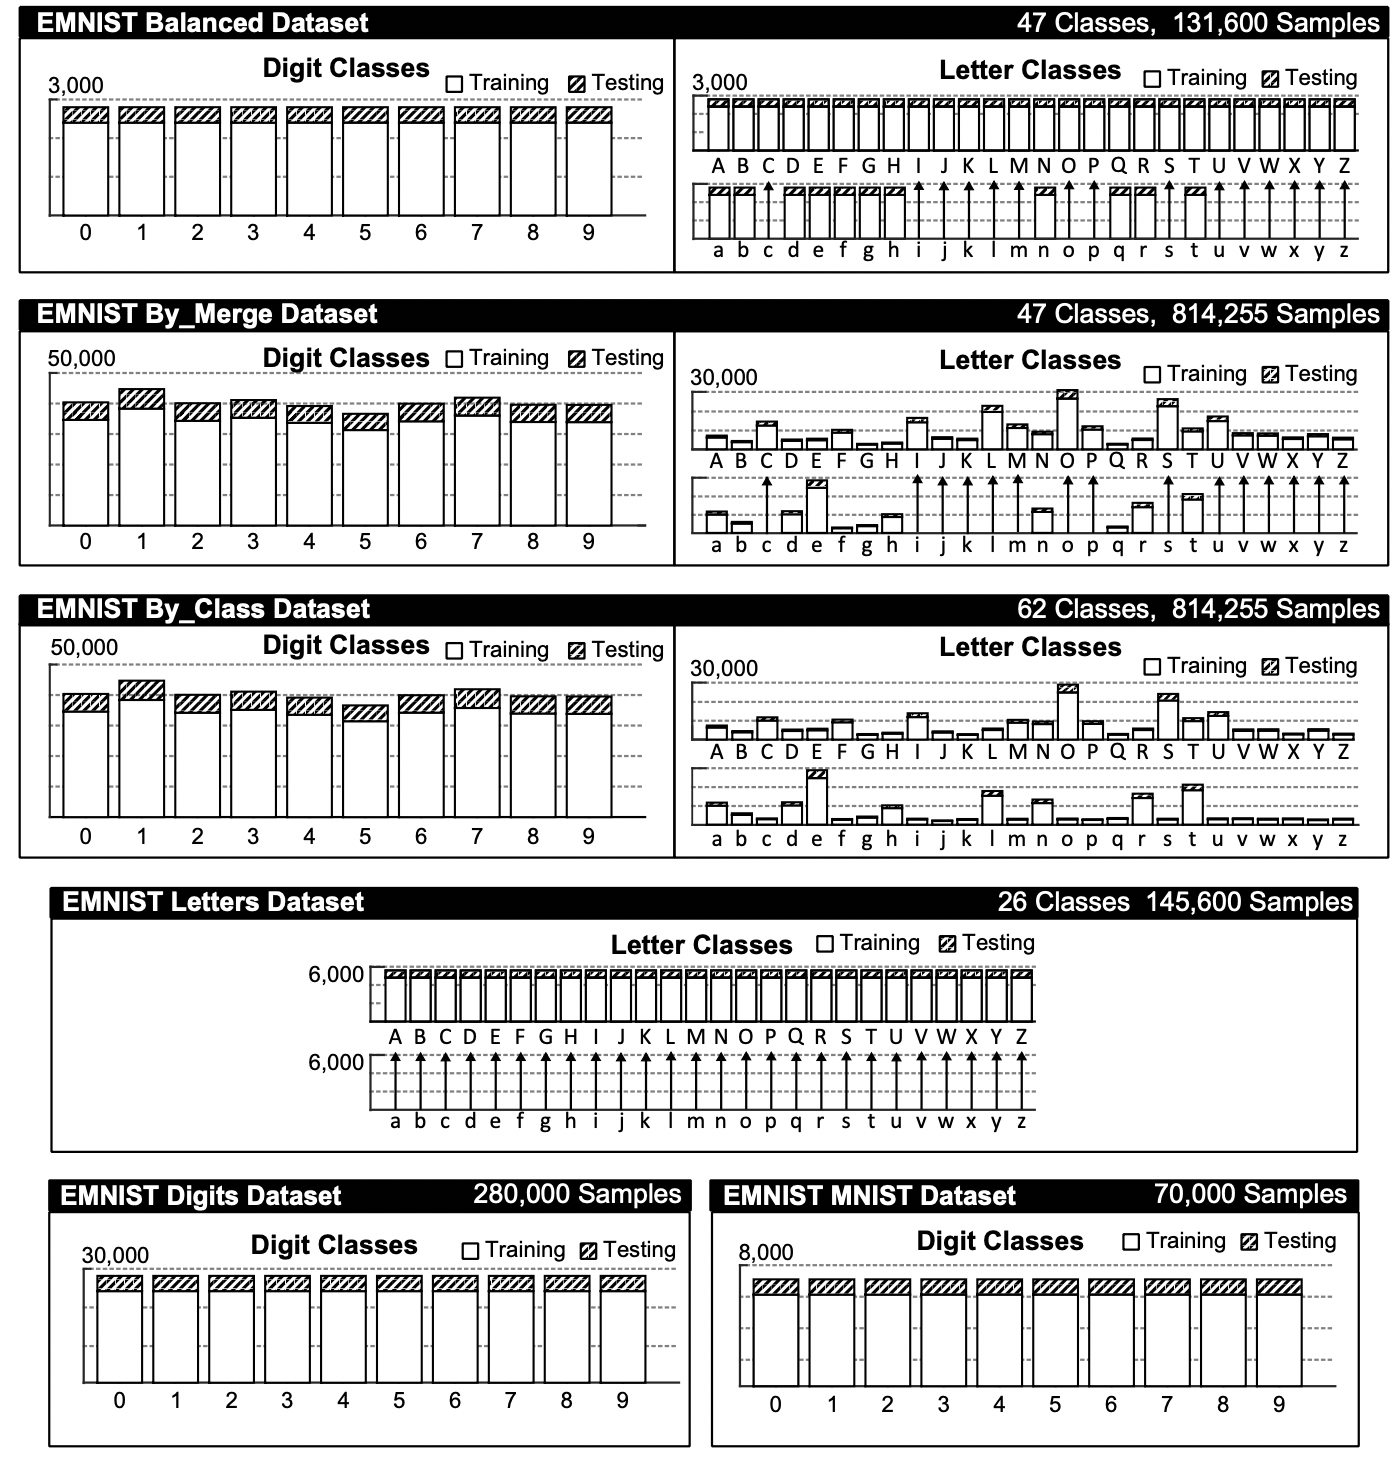
\includegraphics[width=1\linewidth]{images/emnist.jpg}
\caption{\textbf{Visual breakdown of the EMNIST data sets.} The class breakdown, structure and splits of the various data sets in the EMNIST data set are shown. Each data set contains handwritten digits, handwritten letters or a combination of both. The number of samples in each class is shown for each data set and highlights the large variation in the number of samples in the unbalanced data sets. The training and testing split for each class is also shown using either solid or hatched portions of the bar graphs. In the data sets that contain merged classes, a vertical arrow is used to denote the class into which the lowercase letter is merged.}
\label{fig:population}
\end{figure}

In this project, the EMNIST Balanced data set will be used to reduce mis-classification errors due to capital and lower case letters and also has an equal number of samples per class. The EMNIST Balanced includes two main data sets:

\begin{description}[font=$\bullet$~\normalfont\scshape\color{red!50!black}]
  \item \textbf{emnist-balanced-train.csv} - 112,800 images
  \item \textbf{emnist-balanced-test.csv} - 18,800 images
\end{description}

Each image is stored in CSV files using a separated row and 785 columns (first column represents the class labels).

\subsection{Convolutional Neural Network}

A popular deep learning algorithm for classifying and recognizing images is CNN. A class of deep neural networks in this category only require minimal pre-processing. In order for the network to detect ambiguous patterns (edges) in the image more effectively, it inputs the image in the form of separate chunks rather than one pixel at a time. In this project, the proposed architecture for the CNN model with different layers is specifically illustrated below.

\subsubsection{Convolutional Layer}

The convolutional layer is regarded as one of the CNN's fundamental building blocks. It is essential to comprehend that in a CNN, the parameters and channel are made up of a variety of trainable channels or neurons. The receptive field of these channels is constrained. Every channel in the feed-forward process examines the input's dimensions and calculates the dot product of the filter (kernel) pixels and the input pixels. This computation produces a two-dimensional feature map. This allows the system to learn the channels that are created when a particular type of feature is detected at a particular spatial point on the feature map.

In case of the input image \( I \) with height \( H \), width \( W \), and channels \( C = 3\) (red, green and blue) such that \( I \in \mathbb{R}^{H \times W \times C} \), bank of filters/kernels  \( D \) with \( K \in \mathbb{R}^{k_1 \times k_2 \times C \times D} \), and bias \( b \in \mathbb{R}^{D} \), the output from the convolution procedure is as follow: 

\[ (I \ast K)_{ij} = \sum_{m=0}^{k_1 -1}\sum_{n=0}^{k_2 -1}\sum_{c=1}^{C}K_{m,n,c} \cdot I_{i+m,j+n,c} +b_{ij}\]

For the purposes of simplicity, we shall use the case where the input image is grayscale i.e single channel \( C = 1\). The equation above will be transformed to:

\[ (I \ast K)_{ij} = \sum_{m=0}^{k_1 -1}\sum_{n=0}^{k_2 -1}K_{m,n} \cdot I_{i+m,j+n} +b_{ij}\]

The dot product of the input image and kernel is computed by the convolutional layer by moving the kernel over the image to find local features at various locations. Mathematically, we get the large value in the feature maps where the template of the filter is found in the input image. By doing so, the image features that are similar to the kernel are captured. In CNN, filters are considered as weights and are set from the examples during network training via the back propagation algorithm.

\subsubsection{ReLU Layer}

The ReLU or Rectifier Linear Unit activation function, is an additional step to top the Convolution and Neural Network to increase the non-linearity since images are highly non-linear. The function returns 0 if it receives any negative input, but for any positive value  \( x \)  it returns that value back. Therefore it can be mathematically express as

\[ f(x) = max(0,x) \]

or graphically represented 

\begin{figure}[h!]
\centering
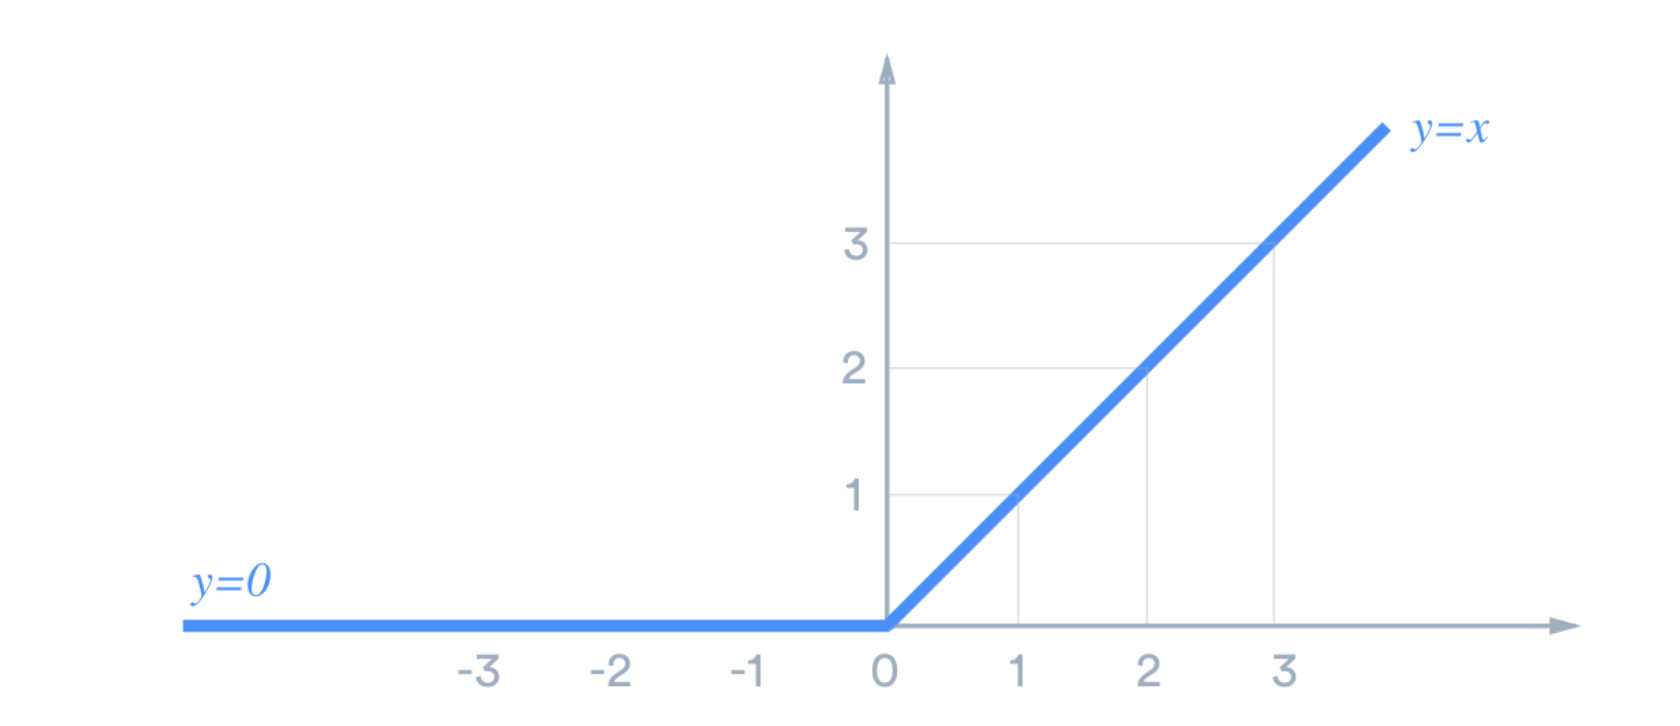
\includegraphics[width=1\linewidth]{images/relu.jpg}
\caption{ReLU activation function}
\label{fig:relu}
\end{figure}

\subsubsection{Pooling Layer}

The size of the feature maps are decreased by pooling layers. As a result, it lessens the quantity of computation done in the network and the number of parameters to learn. In addition, a portion of the feature map created by a convolution layer is summarized by the pooling layer's features. In order to execute additional operations, summarised features rather than precisely positioned features produced by the convolution layer are used. This increases the model's robustness to changes in the features' relative positions in the input image.

Due to their simplicity — they have no parameters to tune — the average pooling and the maximum pooling are frequently utilized in CNNs. The characteristics of the pooling region are all summed up by the average pooling, which is described as

\[ f_{avg} = \frac{1}{N}\sum_{i=1}^{N}|x_i|\]

On the other hand, max pooling selects only the strongest activation in the pooling region,

\[ f_{max} = max\{x_i\}_{i=1}^N\]

\subsubsection{Flatten Layer}

The flattening stage, which is a necessary part of creating a convolutional neural network, is delightfully straightforward.

It entails converting the pooled feature map produced during the pooling process into a one-dimensional vector. Here is an illustration of how this procedure appears

\begin{figure}[h!]
\centering
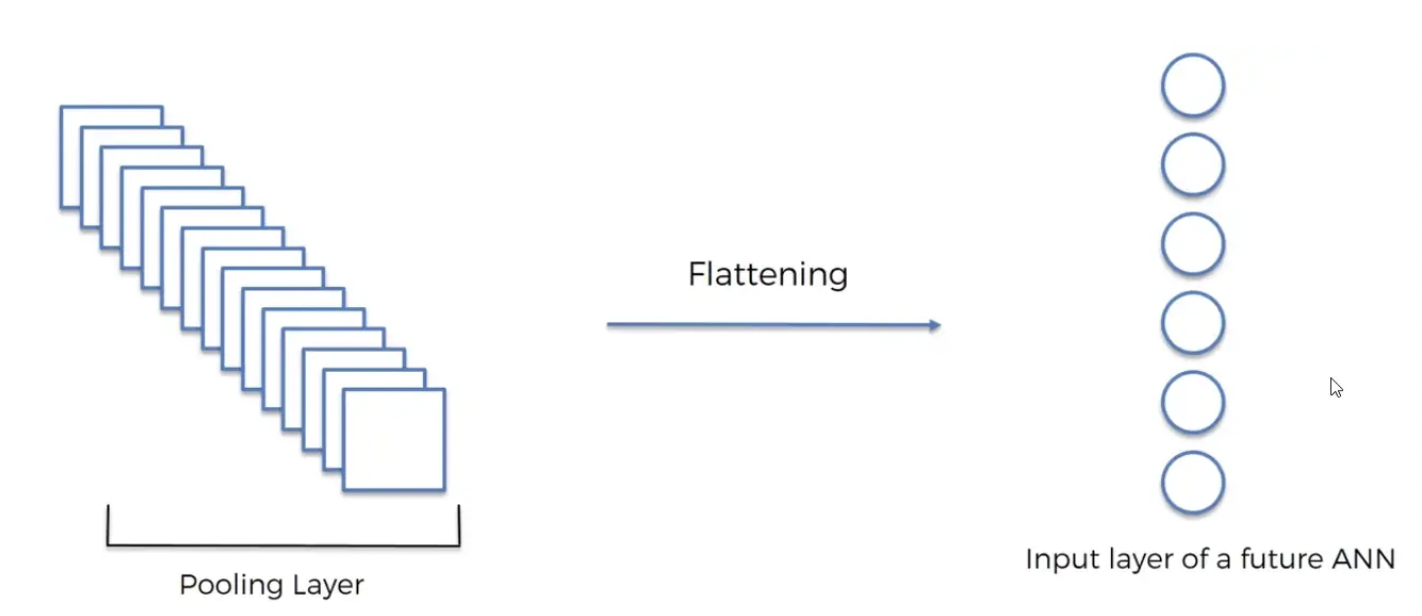
\includegraphics[width=1\linewidth]{images/flatten.jpg}
\caption{\textbf{Flatten layer \cite{b3}.} When you flatten the pooling layers after having multiple pooling layers or pooling layers with several pooled feature maps. As a result, you arrange them in this long column in order, one after the other. And you get a single, enormous vector of inputs for a neural network.}
\label{fig:flatten}
\end{figure}

\subsubsection{Dropout Layer}

The complexity of functions and phenomena that can be described by models with many parameters is astounding. However, this abundance of parameters also implies that the network is free to just describe the data set it was trained on without learning anything new or being able to generalize to new data. Deep neural networks, which include millions of parameters, struggle with the issue of over fitting. By placing a restriction on the parameters and altering the cost function, various regularization strategies are able to solve this issue. Dropout, a more recent development in regularization, differs from other methods in that it alters the network itself.

\begin{figure}[h!]
\centering
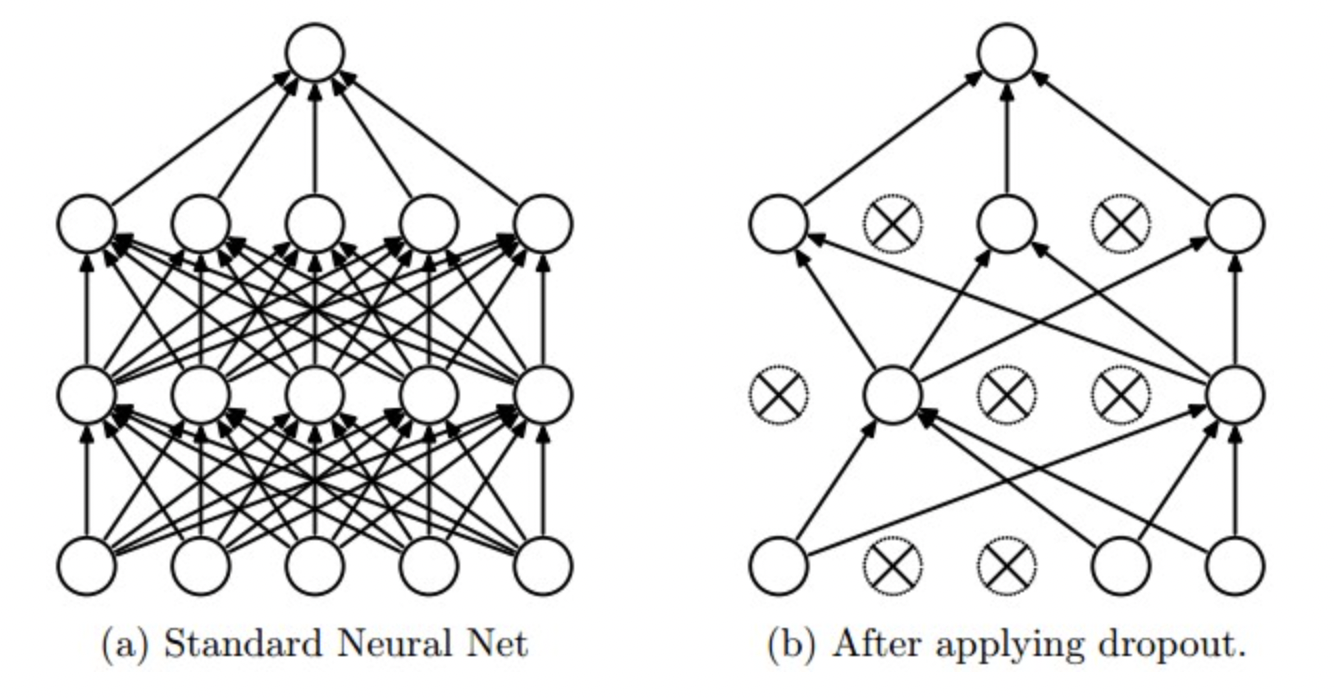
\includegraphics[width=1\linewidth]{images/dropout.jpg}
\caption{\textbf{Dropout layer \cite{b4}.} Dropout works by randomly and temporarily deleting neurons in the hidden layer during the training with probability \( p \).}
\label{fig:dropout}
\end{figure}

Each neuron has a probability of being turned off by probability \( p \). It is possible to model the application of Dropout, during training phase, by transforming the input as:

\[ a = D\odot\sigma(Z)  \]

where \( a \) is the output activation, \( D \) is a vector of Bernoulli variables and \( \sigma(Z) \) is the intermediate activation of the neuron before dropout. A Bernoulli random variable is defined as

\[ f(k,h) = 
\begin{cases}
      p & \text{if $k = 1$}\\
      1 - p & \text{if $k = 0$}
    \end{cases}       \]

\subsubsection{Fully Connected Layer}

Fully-Connected Neural Networks are built from layers of nodes, with each node connected to every other node in the layer before it. With our learned, convolved features as input, this kind of network is put at the very end of our CNN design to create a prediction.

The Fully-Connected layer will take as input a flattened vector of nodes that have been activated in the previous Convolutional and Pooling layers. The vector input will pass through two to three — sometimes more — dense layers and pass through a final activation function before being sent to the output layer. In multi-class classification problem, \textbf{Softmax function} is selected to output a probability distribution which makes it suitable for probabilistic interpretation in classification tasks. Softmax function takes an N-dimensional vector of real numbers and transforms it into a vector of real number in range \( (0,1) \) which add up to 1.

\[ p_i = \frac{e^{z_i}}{\sum_{k=1}^{N} e^z_k}\]

where e is the exponential function, \( p_i (1 \leq i \leq N) \) is the i-th output of the layer and \( z = \{z_1, ..., z_N \} \) is the result of the \( N \) linear combinations of the previous layer’s outputs. The outputs can therefore be read as a likelihood of belonging to each class because they are all included between 0 and 1, and their summation is equal to 1. Finally, the letter is decided upon based on the output with the highest likelihood.

\section{Implementation}

\subsection{Data Pre-processing}
\begin{figure}[h!]
\centering
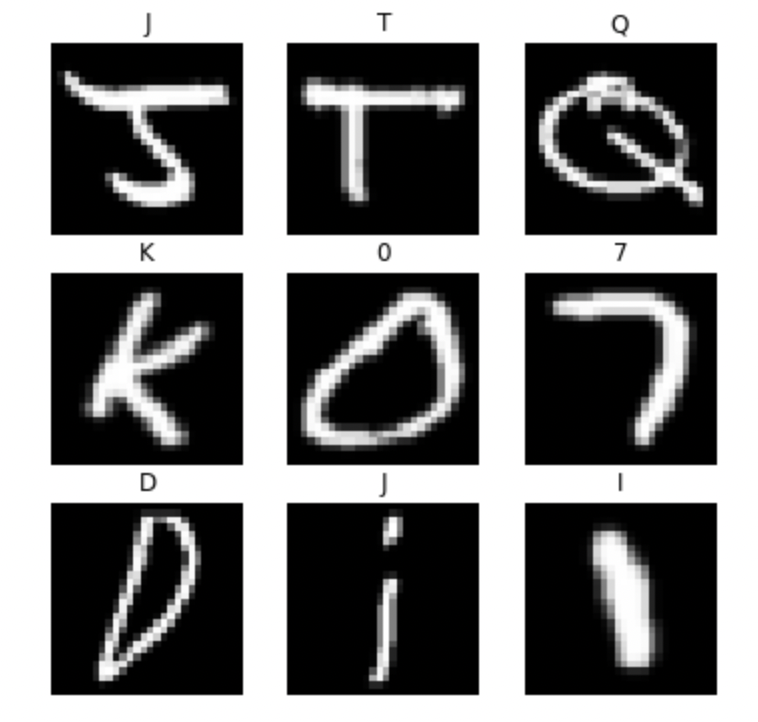
\includegraphics[width=1\linewidth]{images/sample.jpg}
\caption{\textbf{Sample pre-processed data.} The data from the EMNIST balanced data set was adjusted to all be of the same orientation, size, and have normalized pixel intensity values. }
\label{fig:cnn}
\end{figure}
The EMNIST Balanced train and test data sets were first split into separate variables, and the images were flipped and rotated accordingly to all be of the same orientation. The data was then normalized to pixel values out of 255, and reshaped to be 28 x 28 pixels, which helps increase the efficiency of the model by decreasing the complexity of the data. 


\subsection{CNN Model}

Our CNN model contains two convolutional layers, two max pooling layers, a flatten layer, two dense layers and a dropout layer. The first convolutional layer has a 5 x 5 kernel size and 64 filters, which is used to detect the smallest features of the image, such as edges and gradients. The convolutional layer uses relu as its activation function, which helps prevent any potential exponential growth in the computation. The next layer is a max pooling layer with a 2 x 2 pool size, which is used to cut the image size in half to 14 x 14 x 64 features, which helps save time during the computation. The next convolutional layer has a 3 x 3 kernel size and 128 filters, which are used to detect larger features about the image, such as small shapes and corners. Again, relu is used as the activation function. Another max pooling layer is used, with a 2 x 2 pool size, cutting the image size in half again to be 7 x 7 x 128 features. A flatten layer follows, which converts the pooled feature map produced from the first four layers into a one-dimensional vector. The first of the two dense layers is next, which contains 128 units which are used to calculate the weighted average of the 128 features (neurons) obtained in the previous convolutional and pooling layers. A relu activation function is used and all negative values are discarded. A dropout layer is used to nullify half of the features in order to prevent over fitting to help the model perform well with a larger variety of inputs. Finally, the second dense layer with 47 units, one for each class, uses a softmax activation function to pick one of the 47 classes as the output. 

\begin{figure}[h!]
\centering
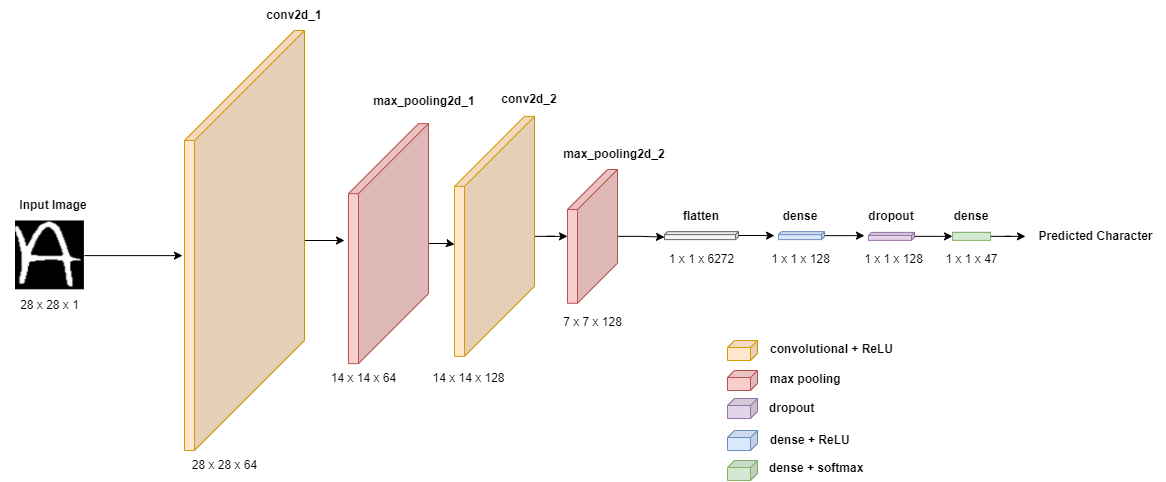
\includegraphics[width=1\linewidth]{images/CNN_Design.jpg}
\caption{\textbf{CNN architecture.} Our CNN Model design consists of two convolution layers, two max pooling layers, a flatten layer, two dense layers, and a dropout layer. The number of filters in each of the convolution layers are listed in the dimensions, with the first convolution consisting of 64 filters, and the second convolution consisting of 128 filters. Each of the max pooling layers have a 2 x 2 pool size,  cutting the image size in half after each application. }
\label{fig:cnn}
\end{figure}

\subsection{Training and Validation Process}

Convolutional and dense layers contain some parameters (also called “weights”) that are determined through an iterative optimization process of minimizing the loss 

\[ L(\theta) = -\frac{1}{N}\sum_{i=1}^{n}\sum_{k=1}^{N}y_{ik}\log{p_{ik}} + \gamma\frac{1}{N_\theta}\sum_{j=1}^{N_\theta}\theta_j^2\]

where \( \theta \) is the vector of size \(N_\theta \) stacking all the parameters to be determined from all the layers, \(i\) is the index of the sample and \(k\) the index of the class. \(p_{ik}\) is the label predicted by the CNN for a sample \(i\). \(y_{ik}\) is the observed label one-hot encoded and log is the algorithm function. The second term of the loss is a L2-regularization term weighted by \(\gamma\) aiming at avoiding overfitting by penalizing high values of parameters. The loss function is optimized iteratively on batches of \(n\) samples using the Adam optimizer \cite{b5}. Table I provides all parameters used in our setup. 

\begin{table}[h!]
\begin{center}
\begin{tabular}{||c c c c||} 
 \hline
 epochs & batch size & optimizer & dropout rate\\ [0.5ex] 
 \hline\hline
 10 & 128 & adam & 0.5 \\ 
 \hline
\end{tabular}
\caption{\label{t1} \textbf{The hyperparameters used in CNN model} }
\end{center}
\end{table}

By Using the architecture implemented in Fig. 6, as well as splitting the original training data set into training and validation data set with the size of 80\% and 20\%, respectively, the CNN model reached an accuracy of 87.57\% on the training set and 88.41\% on the validation set. The training accuracy and learning curve obtained from the training process are illustrated in Fig. 7 and Fig. 8. The error is considered cross-entropy error. 

\begin{figure}[h!]
\centering
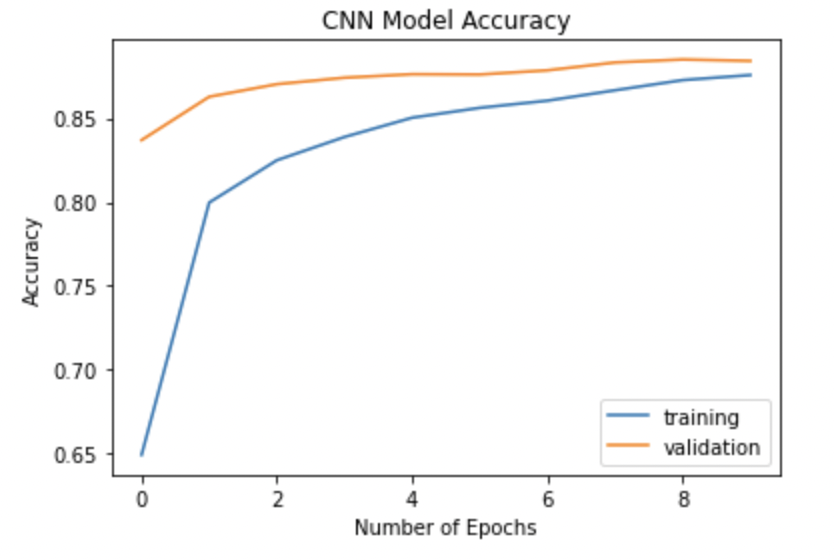
\includegraphics[width=1\linewidth]{images/accuracy.jpg}
\caption{The training accuracy produced by CNN model while training on the EMNIST dataset. The validation accuracy obtained from forward propagation through the validation dataset.}
\label{fig:accuracy}
\end{figure}

\begin{figure}[h!]
\centering
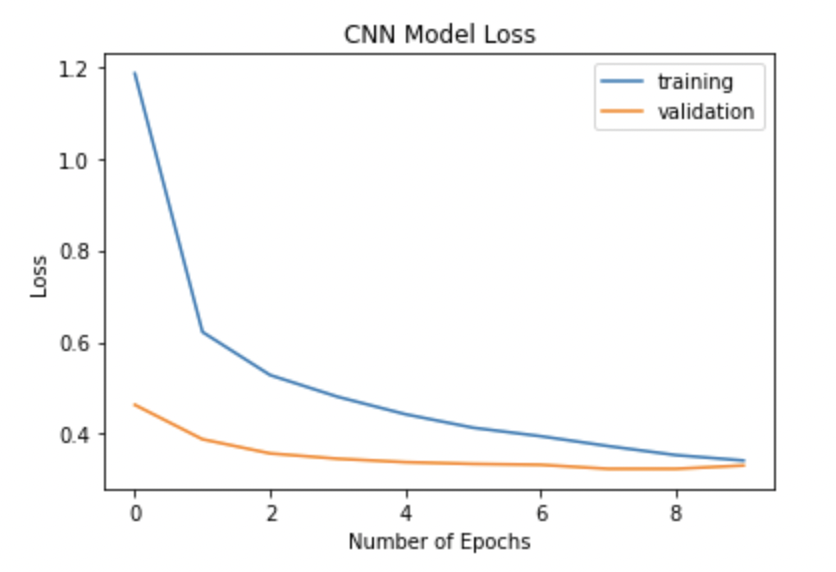
\includegraphics[width=1\linewidth]{images/loss.jpg}
\caption{The loss curve decreases as the model is trained more which depicts the confidence and error while learning the patterns on dataset.}
\label{fig:loss}
\end{figure}

\section{Results}

\subsection{Summary of Training Process}

\begin{table}[h!]
\begin{center}
\begin{tabular}{||c c c ||} 
 \hline
 Epoch \# & Time (s) & Accuracy (\%)\\ [0.5ex] 
 \hline\hline
 1 & 48 & 83.69 \\ 
 \hline
 2 & 47 & 86.28  \\
 \hline
 3 & 47 & 87.03 \\
 \hline
 4 & 49 & 87.41  \\
 \hline
 5 & 48 & 87.62  \\
  \hline
 6 & 48 & 87.60  \\
  \hline
 7 & 48 & 87.85  \\
  \hline
 8 & 48 & 88.32  \\
  \hline
 9 & 48 & 88.50  \\
 	\hline
 10 & 48 & 88.41  \\
 	\hline
  & Total: 7.983 min & Max: 88.50\%  \\[1ex] 
 \hline
\end{tabular}
\caption{\label{t2} \textbf{CNN model training results after 10 epochs} }
\end{center}
\end{table}

\subsection{Predictions on Test Data}

The trained model can be use to recognized handwritten digits and alphabet letters. The performance on the test dataset (18799 data) took approximately 5 sec with an accuracy of 88.30\%. The sample of model's prediction with predicted labels and actual labels for handwritten characters is shown in Fig. 9. In some cases, the model's prediction is wrong. This may happen since the model is not complex enough to capture the in-depth features of the training characters. However, the handwritten characters are unique and it is more difficult, even for human beings, to classify single character (i.e. number 0 and letter o, or number 1 and letter l) instead of the character itself coming in a specific word or sentence.

\begin{figure}[h!]
\centering
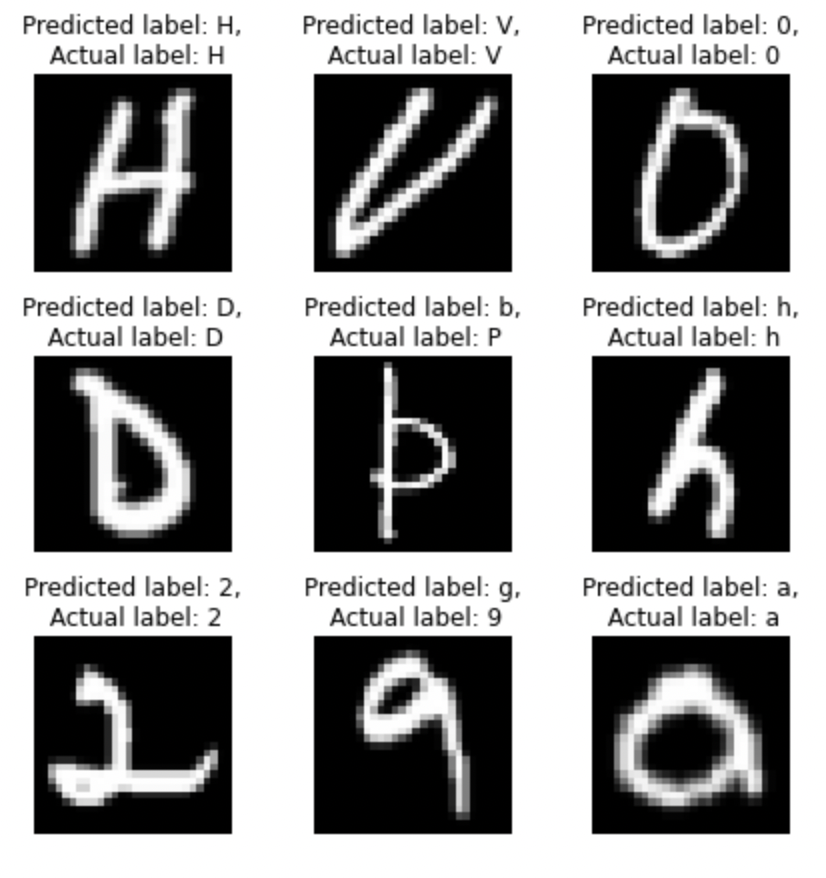
\includegraphics[width=1\linewidth]{images/prediction.jpg}
\caption{Model predictions on test data}
\label{fig:prediction}
\end{figure}

\subsection{Feature Maps}

The sample feature maps produced by the model across different layers are depicted in Fig. 11. The feature maps capture the result of applying randomly eight filters to an input image in Fig. 10. By visualizing the feature maps, we can gain a better understanding of what features the model detects in order to fine tune the model architecture. 

\begin{figure}[h!]
\centering
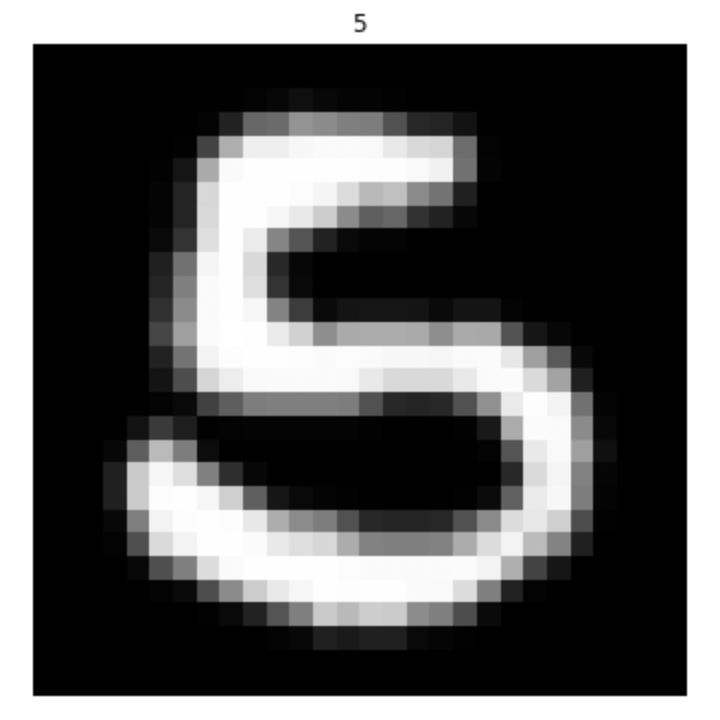
\includegraphics[width=0.8\linewidth]{images/xtrain.jpg}
\caption{Sample input for feature maps visualization}
\label{fig:xtrain}
\end{figure}

\begin{figure*}
  \centering
  \begin{subfigure}{1\linewidth}
    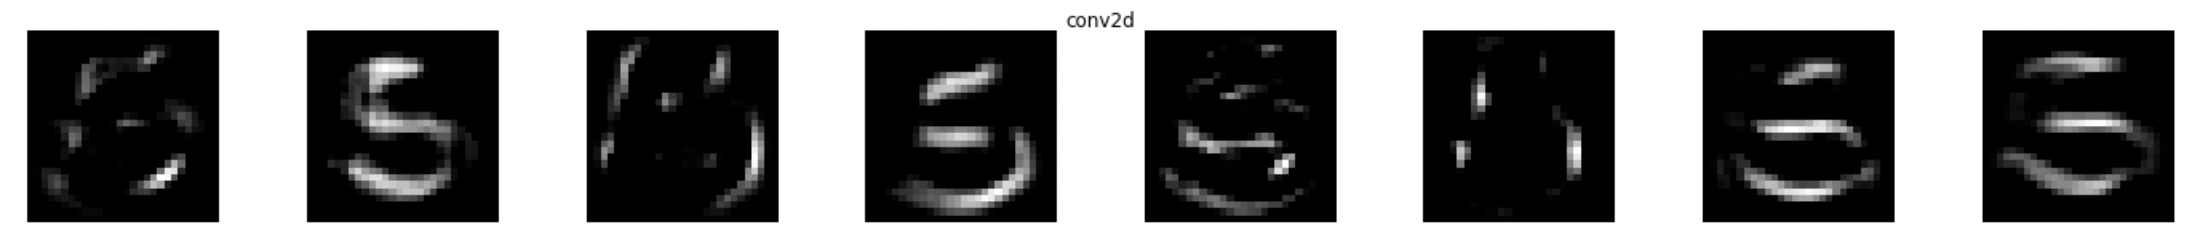
\includegraphics[width=\linewidth]{images/conv2d1.jpg}
     \caption{Layer name: conv2d}
  \end{subfigure}
  \begin{subfigure}{1\linewidth}
    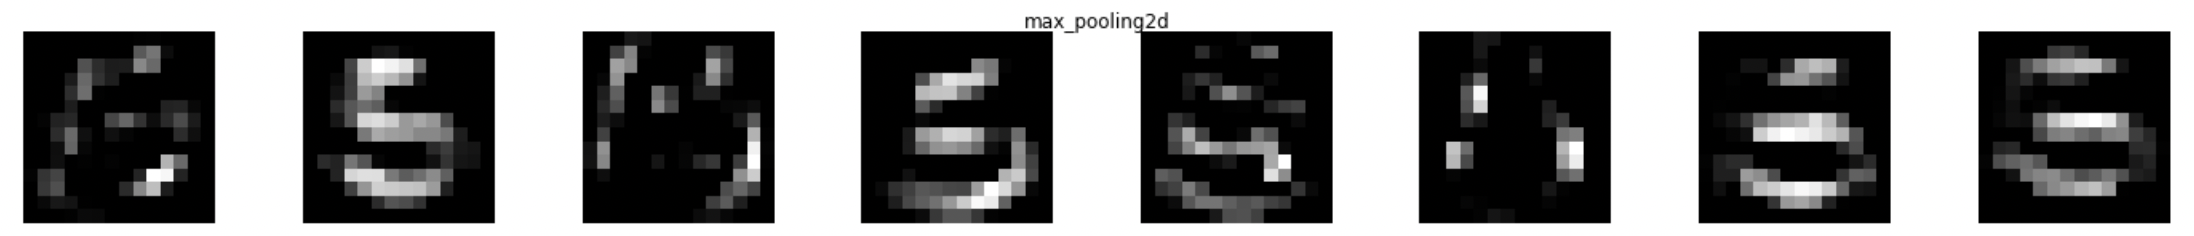
\includegraphics[width=\linewidth]{images/pool2d1.jpg}
    \caption{Layer name: max\_pooling2d}
  \end{subfigure}
  \begin{subfigure}{1\linewidth}
    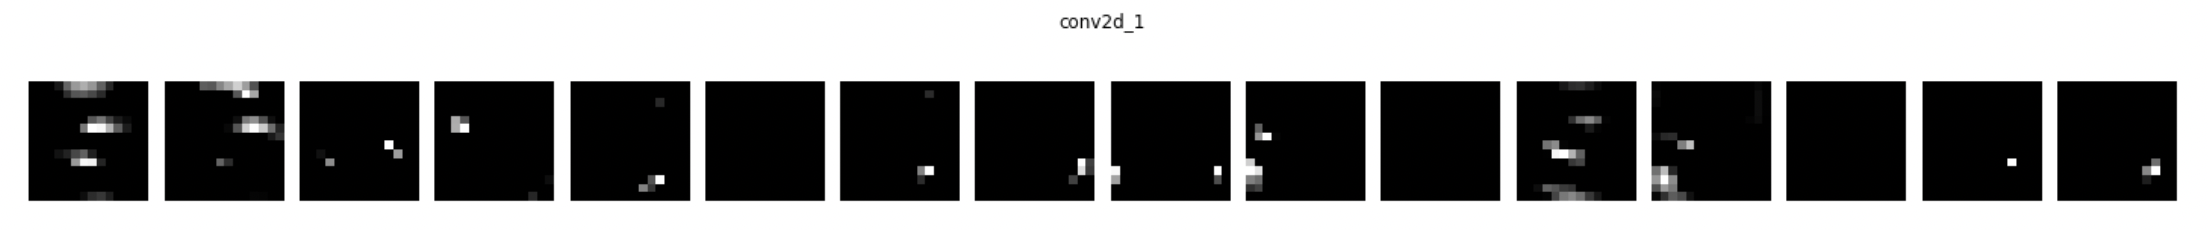
\includegraphics[width=\linewidth]{images/conv2d2.jpg}
    \caption{Layer name: conv2d\_1}
  \end{subfigure}
  \begin{subfigure}{1\linewidth}
    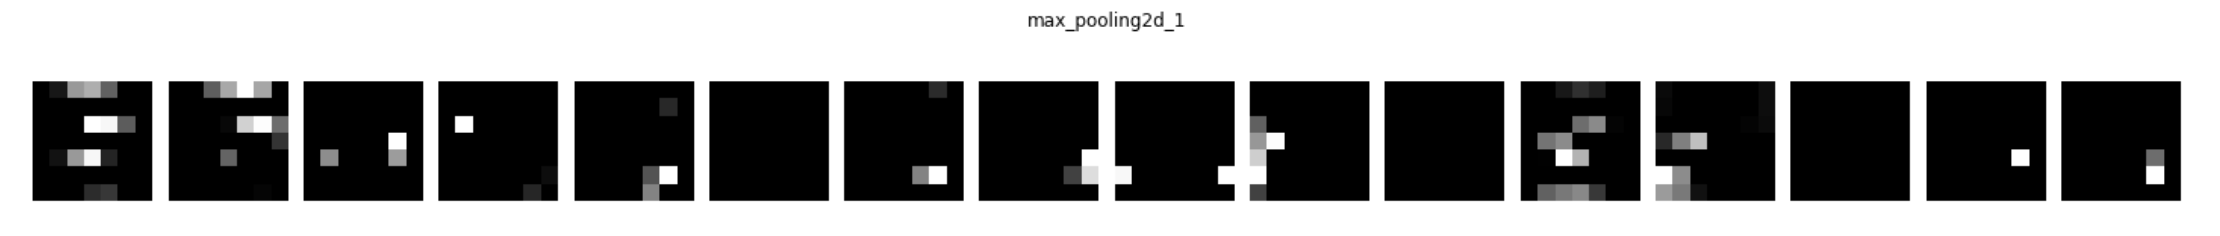
\includegraphics[width=\linewidth]{images/pool2d2.jpg}
    \caption{Layer name: max\_pooling2d\_1}
  \end{subfigure}
  \caption{Feature maps using sample input in Fig. 10. There are only eight sample feature maps shown for each layer due to the limitation on the report length. All feature maps are available in the Python notebook in the GitHub repository provided in the Abstract section.}
  \label{fig:feature maps}
\end{figure*}


\section{Conclusion}

Our CNN model surpassed our goal of 85\% accuracy in under 10 minutes of training time, as it achieved over 88\% accuracy in 8 minutes of training time. The model was able to correctly predict most handwritten characters that were reasonably neat, and most of its inaccurate predictions were due to samples with extremely poor handwriting, or characters that look similar to another character or digit. 

Each group member created a unique CNN model, and the highest performing model was selected as our design. Each group member also evenly contributed to researching, and creating this report. 

\section{Future Work}

Since the performance of the CNN model is quite efficient and accurate, this project can be pursued and developed in different ways. To have an in-depth knowledge about Convolution Neural Network and Deep Learning, an implementation of CNN model from scratch using Python is a good start of applying the theories learned in the project. Another approach is to develop a handwritten detection tool which capable of recognize the text instead of single characters. For a broader picture, multi-class image classification is an important problem since it's the same kind of technology that Tesla uses in their self-driving cars or Airbnb uses in automatically adding information to their listings. 

\begin{thebibliography}{00}

\bibitem{b1} Yamashita, R., Nishio, M., Do, R.K.G. et al. (2018). Convolutional neural networks: an overview and application in radiology. Insights Imaging 9. https://doi.org/10.1007/s13244-018-0639-9  
\bibitem{b2} Cohen, G., Afshar, S., Tapson, J., &amp; van Schaik, A. (2017). EMNIST: Extending mnist to handwritten letters. 2017 International Joint Conference on Neural Networks (IJCNN). https://doi.org/10.1109/ijcnn.2017.7966217                      
\bibitem{b3} Kongsilp, P. (2019, July 22). CNN: Step 3- Flattening. Medium. Retrieved December 16, 2022, from $https://medium.com/@PK_KwanG/cnn-step-2-flattening-50ee0af42e3e$   
\bibitem{b4} Srivastava, N., Hinton, G., Krizhevsky, A., Sutskever, I., &amp; Salakhutdinov, R. (2014, January 1). Dropout: A simple way to prevent neural networks from overfitting: The Journal of Machine Learning Research: Vol 15, no 1. The Journal of Machine Learning Research. Retrieved December 16, 2022, from https://dl.acm.org/doi/abs/10.5555/2627435.2670313              
\bibitem{b5} Kingma, D.P.; Ba, J. Adam: A Method for Stochastic Optimization. arXiv 2014, arXiv:cs.LG/1412.6980.  
\bibitem{b6} Korosov, A., Boulze, H., &amp; Brajard, J. (2021). Convolutional neural networks for classification of sea ice types in sentinel-1 sar data. https://doi.org/10.5194/egusphere-egu21-10580
\bibitem{b7}  McDermott , J. (n.d.). Convolutional Neural Networks - image classification W. Keras. Learn Data Science - Tutorials, Books, Courses, and More. Retrieved December 17, 2022, from   https://www.learndatasci.com/tutorials/convolutional-neural-networks-image-classification/ 
\end{thebibliography}

\end{document}
